\chapter{Cross Section Measurement}

The cross section measurement procedure and results are explained in this section.
After applying selection criteria and kinematic reconstruction, one can count the events to determine
the rate of $t\bar{t}$ production process.

The cross sections were measured double differentially in bins of the kinematic variables of the event.
A binning choice is explained in the first section.
The two dimensional unfolding was applied to correct for the detector effect and fluctuations, which is described
in the second section of this chapter.
The double differential cross sections and their definitions are shown in the last section of the chapter.
% \section{Selection of Binning}\label{sec:binning}

\section{Background Subtraction}
This study is performed as counting the events which fulfill certain criteria (e.g. given in chapter \ref{chapt:event_selection} and 
chapter \ref{chapt:kinReco}). Not all of these events are the $signal events$ originating from the $t\bar{t}$ system decay in dileptonic
channel. The final state, which can be misidentified as $t\bar{t}$, may arise from a different process, called \textit{background}
for the specific measurement. In this analysis the background rates are estimated from the simulation and Subtracted 
from the measured event yields:

\begin{equation}\label{eq:bgsub}
 N^{signal\;measured} = N^{selected} - N^{BG}
\end{equation}

Here the $N^{BG}$ corresponds to the number of background events. It consists of several processes like:

\begin{itemize}
 \item single top production;
 \item Drell-Yan process;
 \item diboson production;
 \item associated $t\bar{t}\;+\; W/Z/\gamma$ production;
 \item associated $W\;+\;jets$ production;
 \item QCD multijet processes.
\end{itemize}

Whereas all the background yields are purely simulated, the rate of the background caused by the Drell-Yan production is 
partially data driven \cite{Chatrchyan:2011nb}. The normalization factor for the simulated Drell-Yan events is determined 
from the comparison of the reconstructed and simulated $Z$-peak. 

After subtracting all the other backgrounds, the number of signal events is multiplied by the factor to cancel the contribution
from the other decay channels of $t\bar{t}$:

\begin{equation}\label{eq:bgsub}
 N^{signal} = N^{signal\;measured} \cdot \frac{N^{t\bar{t} \rightarrow e\mu}_{reco}}{N^{t\bar{t} \rightarrow e\mu}_{reco} + N^{t\bar{t} \rightarrow other}_{reco}}.
\end{equation}

%%%%%%%%%%%%%%%%%%%%%%%%%%%%%%%%%%%%%%%%%%%%
%%%%%%%%%%%%%%%%%%%%%%%%%%%%%%%%%%%%%%%%%%%%
%%%%%%%%%%%%%%%%%%%%%%%%%%%%%%%%%%%%%%%%%%%%
\section{Unfolding of the Experimental Results}\label{sec:unfold}

The events after the background  subtraction \ref{eq:bgsub} are grouped to the bins in different $t$-quark variables. However, a finite precision
of experimental apparatus and reconstruction algorithms may lead to incorrect measurement of kinematic properties of the event.
Thus, some fraction of events may be reconstructed in the wrong bin. To present the results independent of the detector effects,
one needs to correct them back.

The whole problem can be described as

\begin{equation}\label{eq:UnfoldProb}
 \tilde{y}_i = \sum_{j = 1}^{m} A_{ij}\tilde{x}_{j} + b_{i}, \;\;\; 1 \leq i \leq n.
\end{equation}

Here the $\tilde{x}_j$ in $m$ bins is a true distribution, independent of the detector effects, which is the aim of the measurement;
$\tilde{y}_i$ in $n$ bins is a distribution which one gets out of the detector and $A_{ij}$ is a matrix of probabilities describing 
the migration probabilities to different bins on the detector level; $b_{i}$ is the background, or the contribution of other physical
processes, in the bin $i$. However, the pure $\tilde{y}_{i}$ distribution is also not available for the final measurements, because it is
spoiled by the statistical fluctuations, forming the distribution $y_{i}$. The schematic view of the problem is given on the Figure \ref{fig:scUnf}.

\begin{figure}[t]
  \centering
  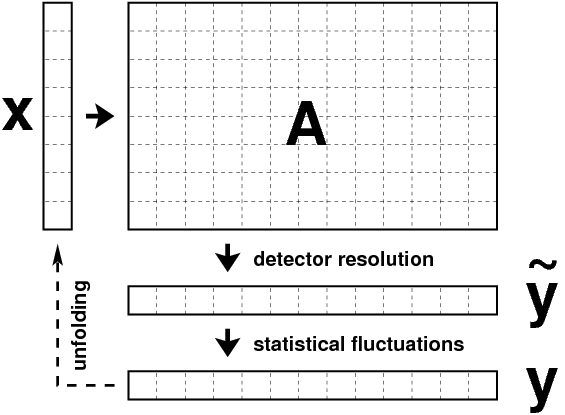
\includegraphics[width=0.4\textwidth]{06_DiffXsec/plots/d12-129f1.png}
  \caption{Schematic view of the problem of migration effects due to the finite precision of the detector and statistical 
  fluctuations. Plot taken from \cite{Schmitt:2012kp}.}
  \label{fig:scUnf}
\end{figure}

The most simple solution would be to take $y_{i}$ instead of $\tilde{y}_{i}$ in eq. \ref{eq:UnfoldProb} and invert
the $A_{ij}$ matrix to obtain $x_{j}$. But it turns out that the statistical fluctuations of $y_{i}$ are greatly 
amplified this way. To minify these fluctuations the \textit{regularisation} procedure is applied.

The process of restoring the true distribution $\tilde{x}_{j}$ from the known distribution $y_{i}$ which was influenced
by the detector effects and statistical fluctuations is called \textit{unfolding}. The TUnfold \cite{Schmitt:2012kp} algorithm was used for the
unfolding in this work.

\subsection{TUnfold Minimization}

The TUnfold algorithm is using the least square minimization method and the Tikhonov regularization \cite{Tikhonov:1963}. One of the crucial 
constrains for a better performance of the method is that the number of degrees of freedom for the minimization ($n - m$) has to be positive,
or $n > m$. This means that the true unfolded distribution $\tilde{x}_j$ will have coarser binning than the measured one, $y_{i}$.

The unfolding algorithm of the TUnfold determines the stationary point or minimum of the Lagrangian:

\begin{align}
 \mathcal{L}(x, \lambda) & = \mathcal{L}_{1} + \mathcal{L}_{2} + \mathcal{L}_{3}, \;\;\;\;\;\;\;\;\;\; \textrm{where}\\
 \mathcal{L}_{1} & = (\mathbf{y} - \mathbf{A}\mathbf{x})^{T} \mathbf{V_{yy}}^{-1}(\mathbf{y} - \mathbf{A}\mathbf{x}),\\
 \mathcal{L}_{2} & = \tau^{2}(\mathbf{x} - f_{b}\mathbf{x_{0}})^{T} (\mathbf{L^{T}L}) (\mathbf{x} - f_{b}\mathbf{x_{0}}), \\
 \mathcal{L}_{3} & = \lambda(Y -\mathbf{e}^{T}\mathbf{x}) \;\;\;\;\;\;\;\;\;\;\;\;\;\;\;\; \textrm{with} \\
 Y & = \sum_{i} y_{i}, \\
 e_{j} & = \sum_{i} A_{ij}.
\end{align}

The bold symbols here correspond to the matrices and vectors.

The term $\mathcal{L}_{1}$ is expected for the minimization. Vectors $\mathbf{y}$, $\mathbf{x}$ and a matrix $\mathbf{A}$ were
described in the previous section. Representing the migrations from and into different bins of $\mathbf{y}$, the matrix $\mathbf{A}$
is often defined from the Monte Carlo\footnote{A matrix $\mathbf{A}$ is
determined from Monte Carlo using the information from the generator particle level and on the reconstructed signal. An extra row is added
to the matrix $\mathbf{A}$ containing the information about the count of Monte Carlo events which were generated in some bin of $\mathbf{x}$,
but were not reconstructed in any of the $\mathbf{y}$ bins.}.
The $\mathbf{V_{yy}}$ is a covariance matrix of $\mathbf{y}$. 

The term $\mathcal{L}_{2}$ is responsible for the regularization. It is reducing the effect of the statistical fluctuations of $\mathbf{y}$
during the search of the stationary point of the Lagrangian $\mathcal{L}$. The $\tau^{2}$ is the regularization strength. Matrix $\mathbf{L}$
represents regularization conditions, having $n$ columns and $n_{R}$ rows which corresponds to $n_{R}$ conditions. $f_{b}$ is a normalization 
factor. In a very simple case $f_{b} = 0$, $\mathbf{L}$ is a unity matrix and $\mathcal{L}_{2} = \tau^{2} \parallel x \parallel^{2}$, which
suppresses the large deviations of $\mathbf{x}$ from zero. In case $f_{b} = 1$, the deviations of $\mathbf{x}$ from $\mathbf{x_{0}}$ are
suppressed. It is very important to choose the optimal regularization strength, as a very weak strength would not damp the fluctuation effects
from $\mathbf{y}$, whereas a very strong one will bias $\mathbf{x}$ towards $f_{b}\mathbf{x}_{0}$. The L-curve method \cite{Hansen00thel-curve} and the minimization
of correlation coefficients \cite{VBlobelT} are implemented in TUnfold for an optimal regularization strength choice. A multidimentional
regularization is possible in TUnfold.

The term $\mathcal{L}_{3}$ is an orthogonal area constrain with a Lagrangian parameter $\lambda$. If $\lambda$ is not set to zero,
which means the area constrain is used, the $\mathbf{x}$ is forced to match the total event count $Y$ correcting for the efficiencies $\mathbf{e}$.
This is used to limit the normalization biases if the data $\mathbf{y}$ follow Poisson's statistics \cite{Cowan98}.

The stationary point of the Lagrangian $\mathcal{L}(\mathbf{x}, \lambda)$ is defined by setting the first derivatives to zero. In case no 
area normalization is performed the Lagrangian $\mathcal{L}$ depends only on $\mathbf{x}$ and $\mathcal{L}_{3}$ term is zero.

\subsubsection{Regularization Studies}

The regularization aims to minimize the fluctuations effects. To check the performance of regularization of the TUnfold, the reconstructed signal
MC sample was unfolded. The outcome of this unfolding should be the generated signal distributions. The number of entries in the reconstructed signal
MC distributions were fluctuated randomly in each bin independently within their statistical uncertainties. These statistical uncertainties were assumed
to be Gaussian. The fluctuations were performed 100 times. Each of the 100 fluctuated distributions was unfolded and the following quantities were checked:

\begin{itemize}
 \item \textbf{RMS over mean error distribution}. All the 100 unfolded distributions are not exactly the same. The statistics in the same bin in each
 distribution will differ. To quantify if this spread of the values is not disagreeing with the statistical uncertainties, one can look at the 
 RMS (root mean square) of the values in a certain bin divided by the mean error of these values. In a perfect case this value should be equal to one.
 The distributions of the RMS over mean errors are shown in the Fig. \ref{fig:RMSovMeanErr}. All the plots show expected behavior.
 
 \item \textbf{Difference between unfolded and generated values.} The mean number of entries in one bin out of 100 fluctuated and unfolded distributions
 is being compared to the number of entries in the corresponding generated distribution. The quantity which evaluates this comparison is
 $\frac{N^{meas}_{mean\:i} - N^{gen}_{i}}{\sigma_{mean\:i}}$. Here $N^(meas)_{mean\:i}$ is the mean number of entries in the bin $i$ out of 100 fluctuated and unfolded distributions,
 $N^{gen}_{i}$ is the number of generated events in the bin $i$ and $\sigma_{mean\:i}$ is the mean error of the fluctuated and unfolded values 
 in the bin $i$. The distributions of this quantifier is shown in the Fig. \ref{fig:DiffovErr}. The overall deviations from zero are not
 higher than 20\%, which means there are no big discrepancies in the unfolding outcome.
 
 \item \textbf{$\tau$ scan}. The regularization strength $\tau$ is determined using L-curve scan and minimization of correlation coefficients for every
 of the 100 fluctuated distributions. The resulting distributions were compared to each other. The regularization strength distributions are shown in
 Fig. ?? and Fig. ?? The regularization strength defined in the L-curve method has two preferred values which shows instability of $\tau$ definition.
 Such phenomenon is not observed in the results of the minimization of correlation coefficients method. The single value of the regularization strength
 is preferred for all the unfolded distributions. Thus, the minimization of correlation coefficients is used for the cross section determination.

\end{itemize}

\begin{figure}[h]
\centering
\begin{subfigure}
  \centering
  \includegraphics[width=0.4\textwidth]{06_DiffXsec/plots/Plots/preunfold/emu/top_rapidity-top_pt/fluctuation_Nominal.png}
\end{subfigure}
\begin{subfigure}
  \centering
  \includegraphics[width=0.4\textwidth]{06_DiffXsec/plots/Plots/preunfold/emu/top_rapidity-top_pt/fluctuation_Nominal.png}
\end{subfigure}
\begin{subfigure}
  \centering
  \includegraphics[width=0.4\textwidth]{06_DiffXsec/plots/Plots/preunfold/emu/top_rapidity-top_pt/fluctuation_Nominal.png}
\end{subfigure}
\begin{subfigure}
  \centering
  \includegraphics[width=0.4\textwidth]{06_DiffXsec/plots/Plots/preunfold/emu/top_rapidity-top_pt/fluctuation_Nominal.png}
\end{subfigure}
\begin{subfigure}
  \centering
  \includegraphics[width=0.4\textwidth]{06_DiffXsec/plots/Plots/preunfold/emu/top_rapidity-top_pt/fluctuation_Nominal.png}
\end{subfigure}
\begin{subfigure}
  \centering
  \includegraphics[width=0.4\textwidth]{06_DiffXsec/plots/Plots/preunfold/emu/top_rapidity-top_pt/fluctuation_Nominal.png}
\end{subfigure}
\caption{RMS over mean error distributions for the 100 fluctuated and unfolded reconstructed MC signal samples. The distributions are
         presented in bins of top $p_{T}$ and $y$ (top left), ...}
\label{fig:RMSovMeanErr}
\end{figure}

\begin{figure}[h]
\centering
\begin{subfigure}
  \centering
  \includegraphics[width=0.4\textwidth]{06_DiffXsec/plots/Plots/preunfold/emu/top_rapidity-top_pt/Diff_Nominal.png}
\end{subfigure}
\begin{subfigure}
  \centering
  \includegraphics[width=0.4\textwidth]{06_DiffXsec/plots/Plots/preunfold/emu/top_rapidity-top_pt/Diff_Nominal.png}
\end{subfigure}
\begin{subfigure}
  \centering
  \includegraphics[width=0.4\textwidth]{06_DiffXsec/plots/Plots/preunfold/emu/top_rapidity-top_pt/Diff_Nominal.png}
\end{subfigure}
\begin{subfigure}
  \centering
  \includegraphics[width=0.4\textwidth]{06_DiffXsec/plots/Plots/preunfold/emu/top_rapidity-top_pt/Diff_Nominal.png}
\end{subfigure}
\begin{subfigure}
  \centering
  \includegraphics[width=0.4\textwidth]{06_DiffXsec/plots/Plots/preunfold/emu/top_rapidity-top_pt/Diff_Nominal.png}
\end{subfigure}
\begin{subfigure}
  \centering
  \includegraphics[width=0.4\textwidth]{06_DiffXsec/plots/Plots/preunfold/emu/top_rapidity-top_pt/Diff_Nominal.png}
\end{subfigure}
\caption{The distributions for the 100 fluctuated and unfolded reconstructed MC signal samples. The distributions are
         presented in bins of top $p_{T}$ and $y$ (top left), ...}
\label{fig:DiffovErr}
\end{figure}


%%%%%%%%%%%%%%%%%%%%%%%%%%%%%%%%%%%%%%%%%%%%
%%%%%%%%%%%%%%%%%%%%%%%%%%%%%%%%%%%%%%%%%%%%
%%%%%%%%%%%%%%%%%%%%%%%%%%%%%%%%%%%%%%%%%%%%
\section{The Double Differential $t\bar{t}$ Production Cross Sections}

\subsection{Cross Section Definition}

After all the corrections are performed, the signal events grouped to different bins are used to define the normalized double differential cross sections
of the $t\bar{t}$ production process:

\begin{equation}\label{eq:ddxsecdef}
 (\frac{1}{\sigma} \frac{d\sigma}{dx\:dy})_{ij} = \frac{1}{\sigma} \cdot \frac{1}{\Delta x_{i}\Delta y_{j}} \cdot \frac{N^{signal}_{ij}}{\epsilon \cdot BR \cdot L}
\end{equation}

Here $\sigma$ is a total cross section, $\epsilon$ is the analysis efficiency, $BR$ is a branching ratio of the $t\bar{t}$ dilepton decay channel and $L$ is the luminosity
collected by the CMS detector, which corresponds to 19.7 $fb^{-1}$. The $x$ and $y$ are the kinematic variables in which the cross sections 
are measured. $i$ and $j$ are the number of bins of the variables $x$ and $y$ with the widths $\Delta x_{i}$ and $\Delta y_{i}$.
The number of corrected and unfolded signal events in the $ij^{\textrm{th}}$ bin is the $N^{signal}_{ij}$.

The total production cross section $\sigma$ is defined as follows:

\begin{equation}
 \sigma = \frac{N^{signal}}{\epsilon \cdot BR \cdot L}.
\end{equation}

\subsection{Phase Space Definition}

The analysis efficiency $\epsilon$ (from the eq. \ref{eq:ddxsecdef}) definition is based on the Monte Carlo simulation and predictions.
It may be defined in two different ways:

\begin{itemize}
 \item In the \textbf{full phase space}, taking to account the selection and the detector efficiencies:
 \begin{equation}\label{eq:epsanal}
  \epsilon = A \cdot \epsilon^{det},
 \end{equation}
 \\
 where $A$ is the \textit{acceptance} which defines the effect of the kinematic selection and $\epsilon^{det}$ is the detector efficiency part.
 The acceptance is measured on the generator level, to exclude the detector effects:
 \\
 \begin{equation}\label{eq:accep}
  A = \frac{N^{PS\;selection}_{gen}}{N^{total}_{gen}}.
 \end{equation}
 \\
 Here $N^{total}_{gen}$ is the total number of all generated $t\bar{t}$ signal events,
 The $N_{gen}^{PS\;selection}$ is the number of generated $t\bar{t}$ signal events which pass the so-called phase space selection for the generated leptons and 
 $b$-jets. This selection fully corresponds to the one applied on the reconstruction level (see sec. \ref{sec:sel}) and requires:
 \begin{itemize}
  \item[--] Leptons with $p_{T} \geq 20\;$GeV and $|\eta| \leq 2.4$;
  \item[--] $b$-jets with $p_{T} \geq 30\;$GeV and $|\eta| \leq 2.4$.
 \end{itemize}
 The acceptance extrapolates the measurements outside the phase space selection criteria to the full phase space, taking to account the theory knowledge underlying in the MC generators.
 \\
 The jets on the generator level are defined analogously to the reconstructed jets (see sec. \ref{sec:JetAlgo}) applying the anti-$k_{T}$ algorithm with the 
 cone of $\Delta R$ = 0.5 on the all stable particles after the hadronization. The jets containing the $B$-hadrons originating from the $b$ quarks from the
 top decay are the $b$-jets used for the phase space selection.
 \\
 The detector resolution is defined by cancellation of the selection effects in the following ratio:
 \\
 \begin{equation}\label{eq:epsdet}
  \epsilon^{det} = \frac{N^{selected}_{reco}}{N^{PS\;selection}_{gen}}.
 \end{equation}
 \\
 Here $N^{selected}_{reco}$ is the number of simulated reconstructed events. Thus, combining the equation \ref{eq:epsanal}, \ref{eq:accep} and \ref{eq:epsdet},
 the analysis efficiency is expressed as following:
 \\
 \begin{equation}
  \epsilon = \frac{N^{selected}_{reco}}{N^{total}_{gen}}.
 \end{equation}
 
 \item In the \textbf{visible phase space}. This efficiency doesn't take to account the selection efficiency, it consists only from the detector efficiency:
 \begin{equation}
  \epsilon = \epsilon^{det} = \frac{N^{selected}_{reco}}{N^{PS\;selection}_{gen}}.
 \end{equation}
 This efficiency definition doesn't rely on the theoretical predictions for the region outside the visible phase space, but the cross section will depend on
 the selection criteria.
\end{itemize}

The cross sections are measured both in visible and full phase spaces, normalized and not normalized to the total cross section $\sigma$. 


\subsection{Double Differential Production Cross Section Measurement}

The production cross sections were measured double differentially in bins of top transverse momentum, rapidity, mass ...
The binning was chosen to have enough entries in each bin so that the error could be treated as Gaussian.


\subsubsection{Cross sections in bins of rapidity and transverse momentum of the top quark}

The production cross section of the $t\bar{t}$ in bins of the rapidity and the transverse momentum of the top quark was
measured in the bins presented in Fig. \ref{fig:CP_2D_y_pt}. This control distribution is also showing the agreement between 
the data and reconstructed MC $t\bar{t}$ signal.

\begin{figure}[t]
  \centering
  \includegraphics[width=0.8\textwidth]{06_DiffXsec/plots/Plots/Nominal/emu/top_rapidity-top_pt/CP_AllBins_top_rapidity_vs_top_pt.pdf}
  \caption{Control distribution of the $y$ of the top quark in bins of the $p_{T}$ of the top quark. The $y$ bins are shown on the top 
  of the plot. The experimental data are marked with the black dots and the reconstructed MC signal is marked with the red area. The 
  different background contributions are also shown. On the bottom part of the plot the ratio between data and MC statistics in each bin
  is presented.}
  \label{fig:CP_2D_y_pt}
\end{figure}

The quality of the reconstruction in each bin can be characterized by the three quantities -- \textit{efficiency} $\epsilon$, \textit{purity} $p$ and
\textit{stability} $s$. They are defined the following way:

\begin{equation}
 \epsilon_{ij} = \frac{N_{ij}^{reco}}{N_{ij}^{gen\:tot}},
\end{equation}

\begin{equation}
 p_{ij} = \frac{N_{ij}^{gen\:and\:reco}}{N_{ij}^{reco}},
\end{equation}

\begin{equation}
 s_{ij} = \frac{N_{ij}^{gen\:and\:reco}}{N_{ij}^{gen}}.
\end{equation}

All of these quantities are determined from the signal MC. Here $ij$ are the bin numbers in the two dimensions. The efficiency 
$\epsilon_{ij}$ is defined as the number of reconstructed events in the bin $ij$, $N_{ij}^{reco}$ divided by the total number of 
the generated events $N_{ij}^{gen\:tot}$. The efficiency contains the effects of the detector acceptance and the reconstruction efficiency.

The purity $p_{ij}$ is the fraction of the number of the events which were generated and reconstructed in the same bin ($N_{ij}^{gen\:and\:reco}$)
and the total number of the reconstructed events in this bin ($N_{ij}^{reco}$). Thus, the purity describes the migrations inside the bin.
The higher the purity is, the less events migrate inside the bin from the other bins. The highest possible purity value is 1.
The migrations of the events to the different bins are caused by the detector resolution and the reconstruction effects.

The stability $s_{ij}$ is the quotient of the number of events generated and reconstructed in the same bin ($N_{ij}^{gen\:and\:reco}$) over the 
number of the generated events inside this bin ($N_{ij}^{gen}$). The stability is quantifying the migrations out of the bin. The higher 
the stability is the less events migrate outside this bin to the other bins. The highest possible stability value is 1.

The efficiency, purity and stability are shown in the Fig. \ref{fig:EPS_2D_y_pt}. The reconstruction efficiency and stability are better on the
high $p_{T}$. Although the high rapidity bins have low reconstruction efficiency, the purity and stability there is higher.

\begin{figure}[t]
  \centering
  \includegraphics[width=0.8\textwidth]{06_DiffXsec/plots/Plots/Nominal/emu/top_rapidity-top_pt/EPS_AllBins_top_rapidity_vs_top_pt.pdf}
  \caption{The efficiency (green circles), purity (blue triangles) and stability (red triangles) in bins of the $p_{T}$ and $y$ of the top quark.}
  \label{fig:EPS_2D_y_pt}
\end{figure}

The Fig. \ref{fig:XS_2D_y_pt} represents the production cross sections of the $t\bar{t}$ pair in bins of top rapidity and top transverse momentum.
The experimentally measured cross sections are compared to the MadGraph+Pythia, Powheg+Pythia, Powheg+Herwig and MC@NLO+Herwig predictions.
The overall good agreement between theory predictions and experimental results is observed. MadGraph+Pythia describes the higher $p_{T}$ bins
worth.

\begin{figure}[t]
\centering
\begin{subfigure}
  \centering
  \includegraphics[width=0.4\textwidth]{06_DiffXsec/plots/Plots/FinalPlot/emu/top_rapidity-top_pt/xSec_top_pt_IN_top_rapidity_0.pdf}
\end{subfigure}
\begin{subfigure}
  \centering
  \includegraphics[width=0.4\textwidth]{06_DiffXsec/plots/Plots/FinalPlot/emu/top_rapidity-top_pt/xSec_top_pt_IN_top_rapidity_1.pdf}
\end{subfigure}
\begin{subfigure}
  \centering
  \includegraphics[width=0.4\textwidth]{06_DiffXsec/plots/Plots/FinalPlot/emu/top_rapidity-top_pt/xSec_top_pt_IN_top_rapidity_2.pdf}
\end{subfigure}
\begin{subfigure}
  \centering
  \includegraphics[width=0.4\textwidth]{06_DiffXsec/plots/Plots/FinalPlot/emu/top_rapidity-top_pt/xSec_top_pt_IN_top_rapidity_3.pdf}
\end{subfigure}
\begin{subfigure}
  \centering
  \includegraphics[width=0.4\textwidth]{06_DiffXsec/plots/Plots/FinalPlot/emu/top_rapidity-top_pt/xSec_top_pt_IN_top_rapidity_4.pdf}
\end{subfigure}
\begin{subfigure}
  \centering
  \includegraphics[width=0.4\textwidth]{06_DiffXsec/plots/Plots/FinalPlot/emu/top_rapidity-top_pt/xSec_top_pt_IN_top_rapidity_5.pdf}
\end{subfigure}
\caption{Normalized differential cross sections in bins of top rapidity and transverse momentum.}
\label{fig:XS_2D_y_pt}
\end{figure}
